% $Header: /cvsroot/latex-beamer/latex-beamer/solutions/generic-talks/generic-ornate-15min-45min.en.tex,v 1.5 2007/01/28 20:48:23 tantau Exp $

\documentclass[12pt]{beamer}
%\documentclass[12pt,handout]{beamer}

% This file is a solution template for:

% - Giving a talk on some subject.
% - The talk is between 15min and 45min long.
% - Style is ornate.



% Copyright 2004 by Till Tantau <tantau@users.sourceforge.net>.
%
% In principle, this file can be redistributed and/or modified under
% the terms of the GNU Public License, version 2.
%
% However, this file is supposed to be a template to be modified
% for your own needs. For this reason, if you use this file as a
% template and not specifically distribute it as part of a another
% package/program, I grant the extra permission to freely copy and
% modify this file as you see fit and even to delete this copyright
% notice.


\mode<presentation>
{
  \usetheme{default}
  % or ...

  \setbeamercovered{transparent}
  % or whatever (possibly just delete it)
}
\setbeamertemplate{navigation symbols}{}%remove navigation symbols


\usepackage[english]{babel}
% or whatever

\usepackage[latin1]{inputenc}
% or whatever

\usepackage{times}
\usepackage{sansmathfonts}
\usepackage[T1]{fontenc}
% Or whatever. Note that the encoding and the font should match. If T1
% does not look nice, try deleting the line with the fontenc.


\title%[Short Paper Title] % (optional, use only with long paper titles)
{}

\subtitle
{} % (optional)

\author%[Author, Another] (optional, use only with lots of authors)
{Ben Holder}%{F.~Author\inst{1} \and S.~Another\inst{2}}
% - Use the \inst{?} command only if the authors have different
%   affiliation.

%\institute[Universities of Somewhere and Elsewhere] % (optional, but mostly needed)
%{
%  \inst{1}%
%  Department of Computer Science\\
%  University of Somewhere
%  \and
%  \inst{2}%
%  Department of Theoretical Philosophy\\
%  University of Elsewhere}
%% - Use the \inst command only if there are several affiliations.
%% - Keep it simple, no one is interested in your street address.

\date%[Short Occasion] % (optional)
{}

\subject{Talks}
% This is only inserted into the PDF information catalog. Can be left
% out.



% If you have a file called "university-logo-filename.xxx", where xxx
% is a graphic format that can be processed by latex or pdflatex,
% resp., then you can add a logo as follows:

% \pgfdeclareimage[height=0.5cm]{university-logo}{university-logo-filename}
% \logo{\pgfuseimage{university-logo}}



% Delete this, if you do not want the table of contents to pop up at
% the beginning of each subsection:
%\AtBeginSubsection[]
%{
%  \begin{frame}<beamer>{Outline}
%    \tableofcontents[currentsection,currentsubsection]
%  \end{frame}
%}


% If you wish to uncover everything in a step-wise fashion, uncomment
% the following command:

%\beamerdefaultoverlayspecification{<+->}

\usepackage{enumerate}
\usepackage{amsmath}
\usepackage{amssymb}
\usepackage[amssymb]{SIunits}
\usepackage{url}
\usepackage{hyperref}
\usepackage[normalem]{ulem}


\setbeamercovered{invisible}

\hypersetup{
    colorlinks=true,     % false: boxed links; true: colored links
    linkcolor=red,       % color of internal links
    citecolor=blue,      % color of links to bibliography
    filecolor=blue,      % color of file links
    urlcolor=blue        % color of external links
}


\begin{document}

%\begin{frame}
%  \titlepage
%\end{frame}

%%%%%%%%%%%%%%%%%%%%%%%%%%%%%%%%%%%%%%
\begin{frame}{Announcements}
	%
	\begin{itemize}
	\addtolength{\itemsep}{0.5\baselineskip}
	\item Grading: I will catch up soon. I'm sorry!
	\item Happy $(\text{perfect square})^3$ day! (and nice pythagoras day!)  (in this perfect-square year!)
	\item \underline{Schedule}:
		%
		\begin{itemize}
		\item[]{\bf Today (Lecture)}: Electromagnetic Spectrum (light) and Blackbody radiation
		\item[]{\bf Tomorrow (Lab)}: ``all the light you cannot see''
		\item[]{\bf Thursday (Discussion)}]: Blackbody radiation and estimating Earth's Temperature
		\item Next Week: Greenhouse Effect I
		\end{itemize}
		%
	\end{itemize}

\end{frame}
%%%%%%%%%%%%%%%%%%%%%%%%%%%%%%%%%%%%%%
\begin{frame}{Today's Reading Quiz (3 min)}


	
\vspace{1cm}

On your own sheet of paper\ldots

\vspace{0.5cm}

{\bf How does the Sun's energy get to the Earth?  How would you describe that energy/energy-transfer, and what are other examples (not the Sun, but same type of energy transfer)?}

\vspace{0.5cm}

Turn in to Blackboard as scanned pdf (or image is fine).

\end{frame}
%%%%%%%%%%%%%%%%%%%%%%%%%%%%%%%%%%%%%%
\begin{frame}{Review: Energy Types, Energy Transfer, Power}

\begin{itemize}
\item[] \underline{Energy Types} (units of Joules = ``J'')
	%
	\begin{itemize}
	\item ``External'': Kinetic ($K$) of object, Potential ($V$) in gravitational or spring ``field''
	\item ``Internal'': Thermal or mechanical kinetic/potential of atoms or internal parts; Chemical; Nuclear
	\item (new today) ``Electromagnetic'': carried by photons/light
	\end{itemize}
	%
\item[] \underline{Energy Transfer Mechanisms} (units: J)
	%
	\begin{itemize}
	\item Mechanical Work: $W = F \times \Delta x$ (force  over a distance)
	\item Heat Conduction: Objects in contact (high $T$ to low)
	\item Convection: fluid motion of internal parts
	\item (today) Radiation: transmission of photons
	\end{itemize}
	%
\item[] \underline{Power}: Energy per time ($P = \frac{E}{\Delta t}$, in units of $\frac{\text{J}}{\text{s}}$)
\item[] \underline{Flux}: Power per area ($F = \frac{E}{\Delta t \times A}$, in units of $\frac{\text{J}}{\text{s} \times \text{m}^2}$)
\end{itemize}

{\tiny See (updated) Discussion from last week: {\bf Energy Info Sheet}}
\end{frame}
%%%%%%%%%%%%%%%%%%%%%%%%%%%%%%%%%%%%%%
\begin{frame}{One last good day for the professor}

Let's sketch an \underline{energy flow diagram} for the professor climbing Mount Ventoux ($h = \unit{1900}{\meter}$).

\vspace{6cm}

First consider the time interval of ``the climb''

\end{frame}
%%%%%%%%%%%%%%%%%%%%%%%%%%%%%%%%%%%%%%
\begin{frame}{One last good day for the professor (part 2)}


\vspace{7cm}

Now consider the time interval of ``the climb'' and ``the previous day's meals'' (2000 calories = \unit{2000}{kcal}; \unit{1}{kcal} = \unit{4200}{\joule})

\end{frame}
%%%%%%%%%%%%%%%%%%%%%%%%%%%%%%%%%%%%%%
\begin{frame}{One last good day for the professor (part 3)}


\begin{columns}[T]
\column{0.35\textwidth}

\vspace{1cm}

{\bf Q: Where is all of the food energy going?}\\[12pt]

{\bf A: Turns out the professor is a light bulb.}

\vspace{1.cm}

Any object with a temperature ($>\unit{0}{\kelvin}$) emits electromagnetic radiation

\vfill

{\tiny (There is also similar heat losses}\\[-8pt]
{\tiny  due to convection/conduction.)}

\column{0.6\textwidth}

\begin{center}
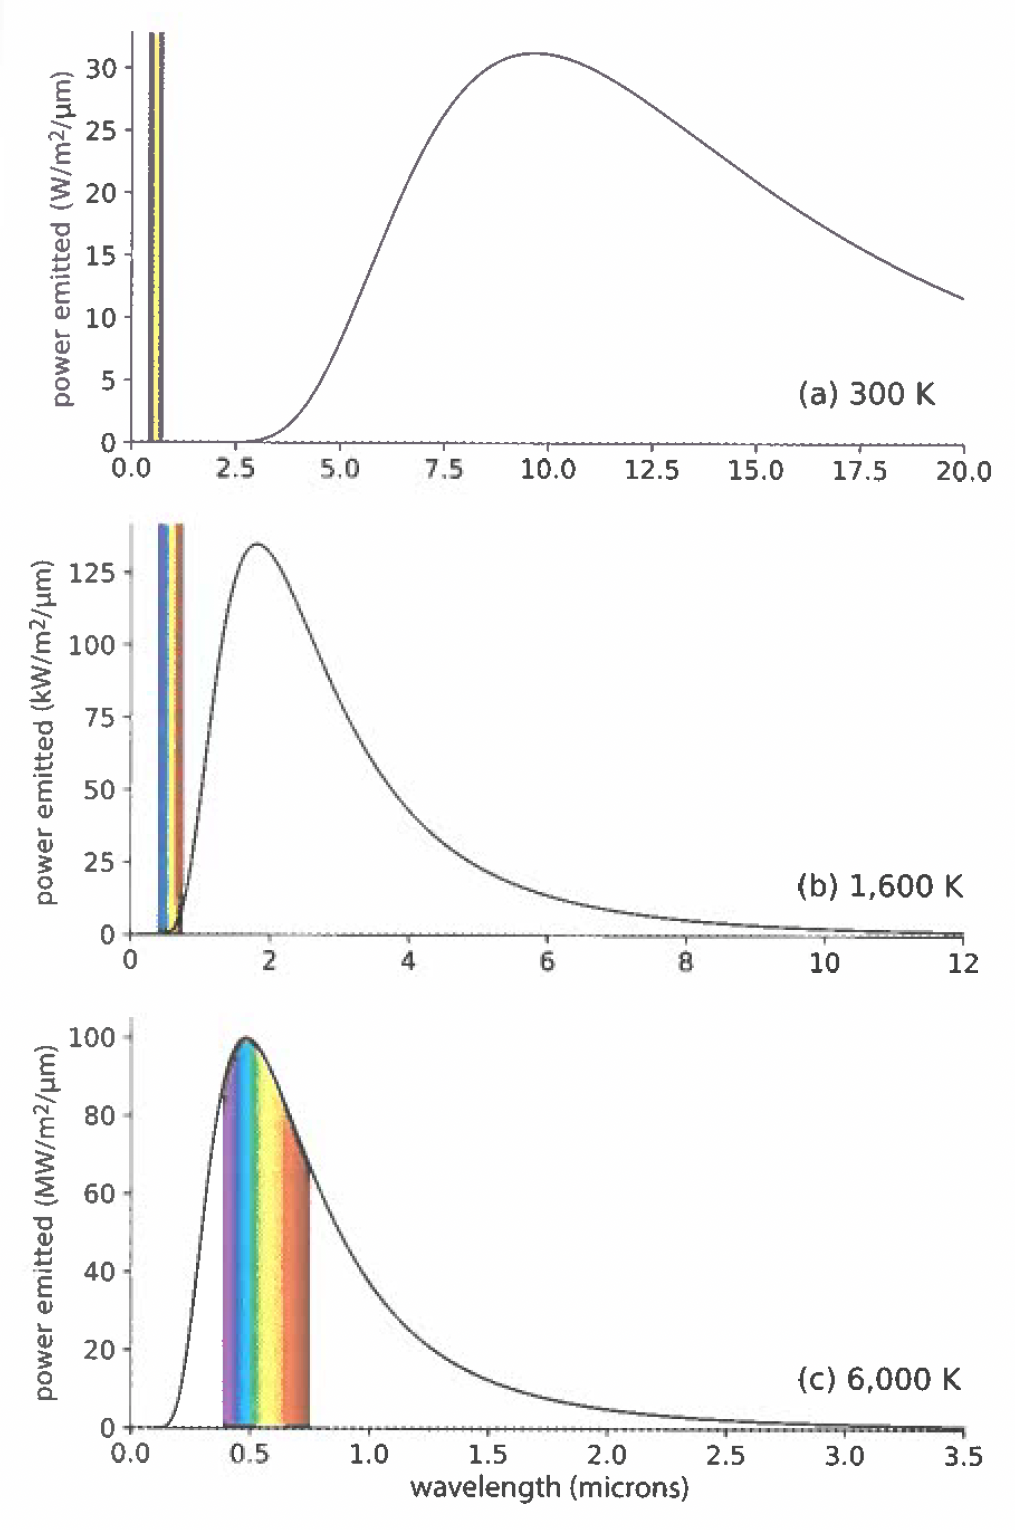
\includegraphics[width=0.8\textwidth]{images/dessler_fig3-2.png}
\end{center}
\end{columns}

\end{frame}
%%%%%%%%%%%%%%%%%%%%%%%%%%%%%%%%%%%%%%
\begin{frame}{Electromagnetic Radiation (light!)}

\begin{center}
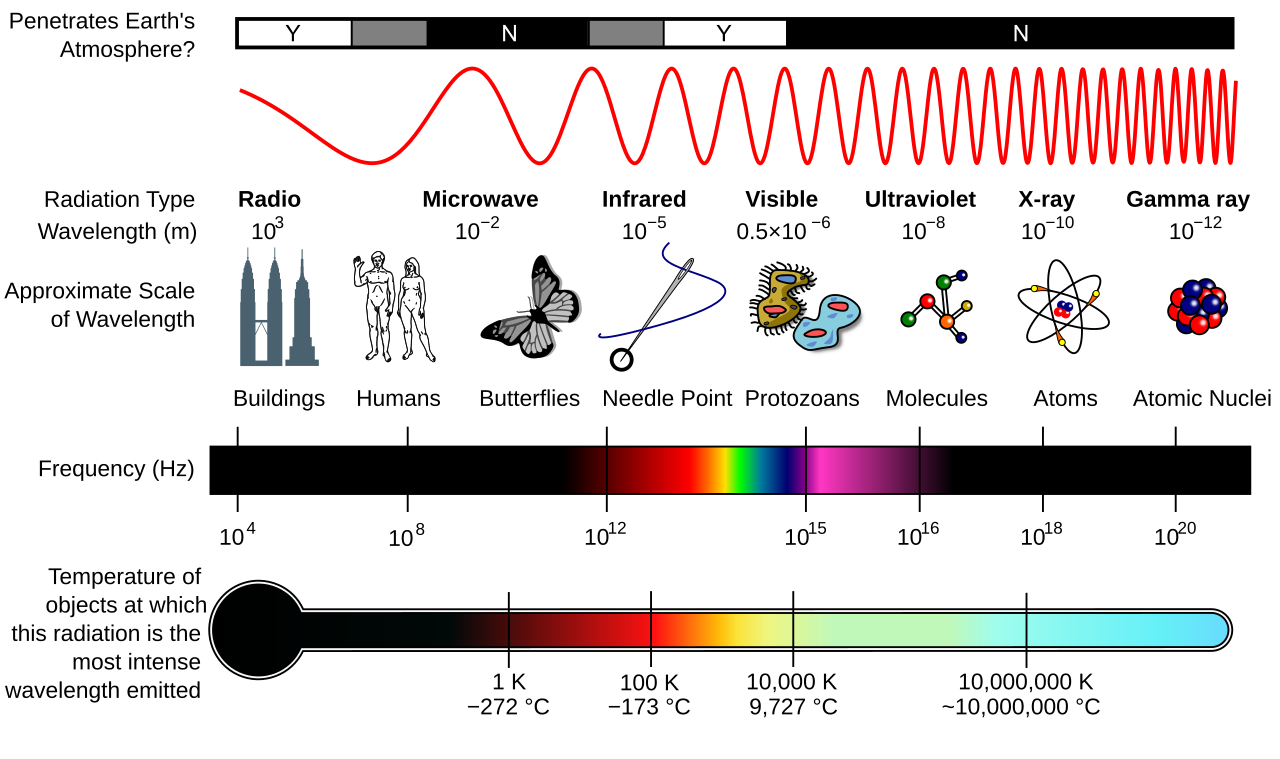
\includegraphics[width=\textwidth]{images/EM_Spectrum_Properties_edit.svg.png}
\end{center}
\hfill {\tiny Wikimedia}

\end{frame}
%%%%%%%%%%%%%%%%%%%%%%%%%%%%%%%%%%%%%%
\begin{frame}{Equations for Blackbody Radiation}


\begin{columns}[T]
\column{0.35\textwidth}

\vspace{1cm}

\underline{Wien's Law}
\begin{equation*}
\lambda_\text{peak} = \frac{\unit{2900}{\micro\meter \cdot \kelvin}}{T}
\end{equation*}


\underline{Stefan-Boltz.\ Law (total flux)}
\begin{equation*}
F = \left( 6 \times 10^{-8} \, \frac{\text{J}/\text{s}}{\text{m}^2 \cdot \text{K}}\right) T^4
\end{equation*}


\underline{Peak ``Spectral Flux''}
\begin{equation*}
F_\lambda = \frac{F}{1.5 \times \lambda_\text{peak}}
\end{equation*}


\column{0.6\textwidth}

\begin{center}
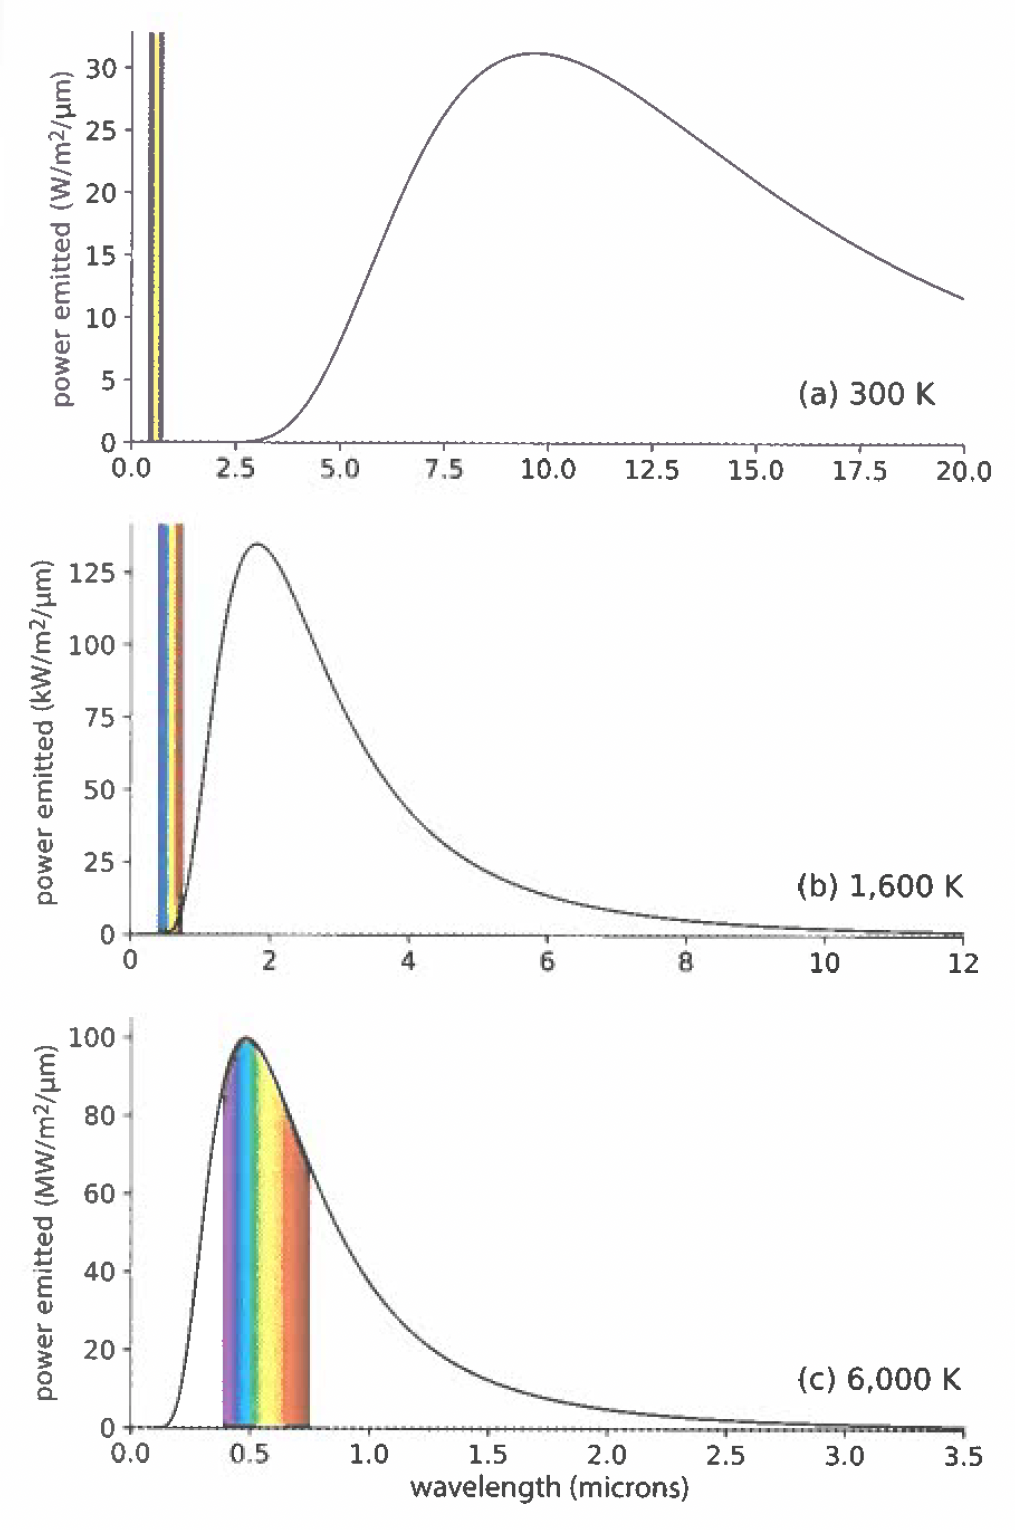
\includegraphics[width=0.8\textwidth]{images/dessler_fig3-2.png}
\end{center}
\end{columns}

\end{frame}
%%%%%%%%%%%%%%%%%%%%%%%%%%%%%%%%%%%%%%
\begin{frame}{Graphing Bb Radiation}

Let's graph (on the log-log paper provided) the Bb radiation of three objects:
	%
	\begin{itemize}
	\item Sun ($T = \unit{6000}{\kelvin}$)
	\item Human ($T = \unit{310}{\kelvin}$)
	\item Liquid Nitrogen ($T = \unit{77}{\kelvin}$)
	\end{itemize}
	%
We use Wien's law and the ``spectral flux'' peak, as well as a 10\% width of $(\lambda / 2, \lambda \times 3)$.

\end{frame}
%%%%%%%%%%%%%%%%%%%%%%%%%%%%%%%%%%%%%%
\end{document}
